\documentclass[11pt]{article}

\usepackage{../theory}

\begin{document}

\coverpage{2}

\newpage
\section*{Problem 1}
\subsection*{1.1}
Give state diagrams of DFAs recognizing the following languages. The alphabet is $\{0, 1\}$. 
$$ A_1 = \{ w \mid w \text{ contains the substring } 0101\}$$
$$ A_2 = \{ w \mid w \text{ does not contain the substring } 110 \}$$
\newline

\noindent
{\bf Proof: } We begin by giving the DFA for $A_1$:

% DFA for A_1 is pictured here
\begin{center}
	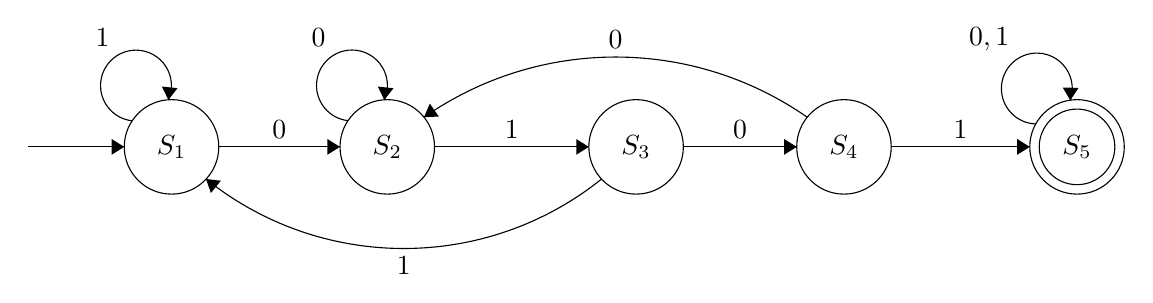
\begin{tikzpicture}[scale=0.2]
	\tikzstyle{every node}+=[inner sep=0pt]
	\draw [black] (13.6,-28.4) circle (3);
	\draw (13.6,-28.4) node {$S_1$};
	\draw [black] (27.3,-28.4) circle (3);
	\draw (27.3,-28.4) node {$S_2$};
	\draw [black] (43.1,-28.4) circle (3);
	\draw (43.1,-28.4) node {$S_3$};
	\draw [black] (71.1,-28.4) circle (3);
	\draw (71.1,-28.4) node {$S_5$};
	\draw [black] (71.1,-28.4) circle (2.4);
	\draw [black] (56.3,-28.4) circle (3);
	\draw (56.3,-28.4) node {$S_4$};
	\draw [black] (4.5,-28.4) -- (10.6,-28.4);
	\fill [black] (10.6,-28.4) -- (9.8,-27.9) -- (9.8,-28.9);
	\draw [black] (16.6,-28.4) -- (24.3,-28.4);
	\fill [black] (24.3,-28.4) -- (23.5,-27.9) -- (23.5,-28.9);
	\draw (20.45,-27.9) node [above] {$0$};
	\draw [black] (30.3,-28.4) -- (40.1,-28.4);
	\fill [black] (40.1,-28.4) -- (39.3,-27.9) -- (39.3,-28.9);
	\draw (35.2,-27.9) node [above] {$1$};
	\draw [black] (46.1,-28.4) -- (53.3,-28.4);
	\fill [black] (53.3,-28.4) -- (52.5,-27.9) -- (52.5,-28.9);
	\draw (49.7,-27.9) node [above] {$0$};
	\draw [black] (59.3,-28.4) -- (68.1,-28.4);
	\fill [black] (68.1,-28.4) -- (67.3,-27.9) -- (67.3,-28.9);
	\draw (63.7,-27.9) node [above] {$1$};
	\draw [black] (11.112,-26.745) arc (264.09973:-23.90027:2.25);
	\draw (9.22,-22.06) node [above] {$1$};
	\fill [black] (13.4,-25.42) -- (13.98,-24.67) -- (12.99,-24.57);
	\draw [black] (24.818,-26.736) arc (263.89012:-24.10988:2.25);
	\draw (22.94,-22.05) node [above] {$0$};
	\fill [black] (27.11,-25.42) -- (27.69,-24.68) -- (26.7,-24.57);
	\draw [black] (40.907,-30.443) arc (-51.29934:-128.70066:20.084);
	\fill [black] (15.79,-30.44) -- (16.1,-31.33) -- (16.73,-30.55);
	\draw (28.35,-35.35) node [below] {$1$};
	\draw [black] (29.632,-26.517) arc (124.87895:55.12105:21.278);
	\fill [black] (29.63,-26.52) -- (30.57,-26.47) -- (30,-25.65);
	\draw (41.8,-22.19) node [above] {$0$};
	\draw [black] (68.491,-26.944) arc (268.56764:-19.43236:2.25);
	\draw (65.52,-22.34) node [above] {$0,1$};
	\fill [black] (70.67,-25.44) -- (71.19,-24.66) -- (70.19,-24.63);
	\end{tikzpicture}
\end{center}

\noindent And now we show the DFA for $A_2$:

% DFA for A_2
\begin{center}
	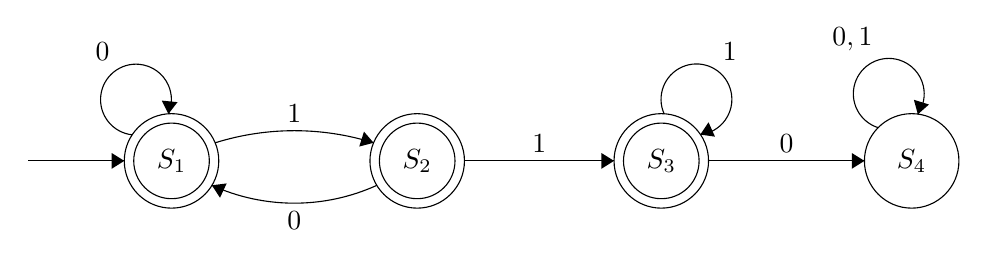
\begin{tikzpicture}[scale=0.2]
	\tikzstyle{every node}+=[inner sep=0pt]
	\draw [black] (13.6,-28.4) circle (3);
	\draw (13.6,-28.4) node {$S_1$};
	\draw [black] (13.6,-28.4) circle (2.4);
	\draw [black] (29.2,-28.4) circle (3);
	\draw (29.2,-28.4) node {$S_2$};
	\draw [black] (29.2,-28.4) circle (2.4);
	\draw [black] (44.7,-28.4) circle (3);
	\draw (44.7,-28.4) node {$S_3$};
	\draw [black] (44.7,-28.4) circle (2.4);
	\draw [black] (60.6,-28.4) circle (3);
	\draw (60.6,-28.4) node {$S_4$};
	\draw [black] (4.5,-28.4) -- (10.6,-28.4);
	\fill [black] (10.6,-28.4) -- (9.8,-27.9) -- (9.8,-28.9);
	\draw [black] (11.112,-26.745) arc (264.11101:-23.88899:2.25);
	\draw (9.22,-22.06) node [above] {$0$};
	\fill [black] (13.4,-25.42) -- (13.98,-24.67) -- (12.98,-24.57);
	\draw [black] (16.368,-27.252) arc (107.41125:72.58875:16.818);
	\fill [black] (26.43,-27.25) -- (25.82,-26.54) -- (25.52,-27.49);
	\draw (21.4,-25.98) node [above] {$1$};
	\draw [black] (32.2,-28.4) -- (41.7,-28.4);
	\fill [black] (41.7,-28.4) -- (40.9,-27.9) -- (40.9,-28.9);
	\draw (36.95,-27.9) node [above] {$1$};
	\draw [black] (47.7,-28.4) -- (57.6,-28.4);
	\fill [black] (57.6,-28.4) -- (56.8,-27.9) -- (56.8,-28.9);
	\draw (52.65,-27.9) node [above] {$0$};
	\draw [black] (26.64,-29.951) arc (-65.57385:-114.42615:12.672);
	\fill [black] (16.16,-29.95) -- (16.68,-30.74) -- (17.1,-29.83);
	\draw (21.4,-31.59) node [below] {$0$};
	\draw [black] (44.882,-25.417) arc (204.23958:-83.76042:2.25);
	\draw (49.05,-22.04) node [above] {$1$};
	\fill [black] (47.18,-26.73) -- (48.11,-26.86) -- (47.7,-25.95);
	\draw [black] (58.482,-26.292) arc (252.86177:-35.13823:2.25);
	\draw (56.84,-21.45) node [above] {$0,1$};
	\fill [black] (60.99,-25.44) -- (61.7,-24.82) -- (60.74,-24.52);
	\end{tikzpicture}
\end{center}

\noindent So we have the DFAs for languages $A_1$ and $A_2$.

$\hfill \Box$

\subsection*{1.2}
Give state diagrams of the NFAs with the specified number of states recognizing each of the following languages. The alphabet is $\{0, 1\}$.
$$ B_1 = \{ w \mid w \text{ contains the substring 0101} \} \text{ using 5 states}$$
$$ B_2 = \{ w \mid w \text{ contains an even number of 0s, or exactly two 1s} \} \text{ with 6 states}$$

\noindent
{\bf Proof: } For $B_1$, we use the same DFA as for $A_1$ (since every DFA is an NFA). It is displayed below.

\begin{center}
	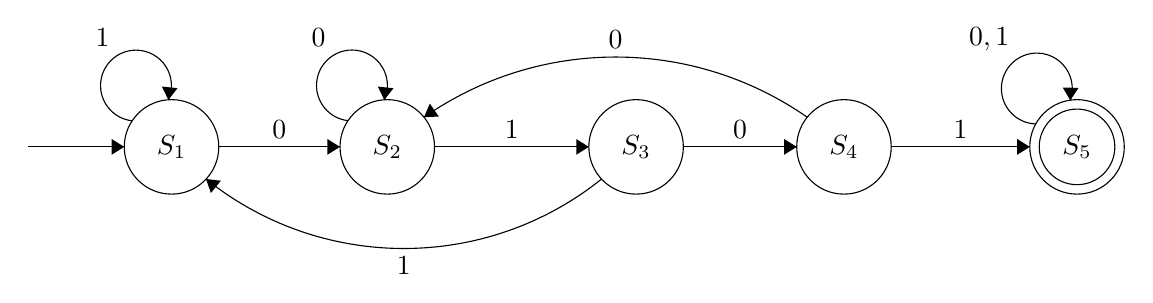
\begin{tikzpicture}[scale=0.2]
	\tikzstyle{every node}+=[inner sep=0pt]
	\draw [black] (13.6,-28.4) circle (3);
	\draw (13.6,-28.4) node {$S_1$};
	\draw [black] (27.3,-28.4) circle (3);
	\draw (27.3,-28.4) node {$S_2$};
	\draw [black] (43.1,-28.4) circle (3);
	\draw (43.1,-28.4) node {$S_3$};
	\draw [black] (71.1,-28.4) circle (3);
	\draw (71.1,-28.4) node {$S_5$};
	\draw [black] (71.1,-28.4) circle (2.4);
	\draw [black] (56.3,-28.4) circle (3);
	\draw (56.3,-28.4) node {$S_4$};
	\draw [black] (4.5,-28.4) -- (10.6,-28.4);
	\fill [black] (10.6,-28.4) -- (9.8,-27.9) -- (9.8,-28.9);
	\draw [black] (16.6,-28.4) -- (24.3,-28.4);
	\fill [black] (24.3,-28.4) -- (23.5,-27.9) -- (23.5,-28.9);
	\draw (20.45,-27.9) node [above] {$0$};
	\draw [black] (30.3,-28.4) -- (40.1,-28.4);
	\fill [black] (40.1,-28.4) -- (39.3,-27.9) -- (39.3,-28.9);
	\draw (35.2,-27.9) node [above] {$1$};
	\draw [black] (46.1,-28.4) -- (53.3,-28.4);
	\fill [black] (53.3,-28.4) -- (52.5,-27.9) -- (52.5,-28.9);
	\draw (49.7,-27.9) node [above] {$0$};
	\draw [black] (59.3,-28.4) -- (68.1,-28.4);
	\fill [black] (68.1,-28.4) -- (67.3,-27.9) -- (67.3,-28.9);
	\draw (63.7,-27.9) node [above] {$1$};
	\draw [black] (11.112,-26.745) arc (264.09973:-23.90027:2.25);
	\draw (9.22,-22.06) node [above] {$1$};
	\fill [black] (13.4,-25.42) -- (13.98,-24.67) -- (12.99,-24.57);
	\draw [black] (24.818,-26.736) arc (263.89012:-24.10988:2.25);
	\draw (22.94,-22.05) node [above] {$0$};
	\fill [black] (27.11,-25.42) -- (27.69,-24.68) -- (26.7,-24.57);
	\draw [black] (40.907,-30.443) arc (-51.29934:-128.70066:20.084);
	\fill [black] (15.79,-30.44) -- (16.1,-31.33) -- (16.73,-30.55);
	\draw (28.35,-35.35) node [below] {$1$};
	\draw [black] (29.632,-26.517) arc (124.87895:55.12105:21.278);
	\fill [black] (29.63,-26.52) -- (30.57,-26.47) -- (30,-25.65);
	\draw (41.8,-22.19) node [above] {$0$};
	\draw [black] (68.491,-26.944) arc (268.56764:-19.43236:2.25);
	\draw (65.52,-22.34) node [above] {$0,1$};
	\fill [black] (70.67,-25.44) -- (71.19,-24.66) -- (70.19,-24.63);
	\end{tikzpicture}
\end{center}

\noindent We now give the NFA for $B_2$:

\begin{center}
	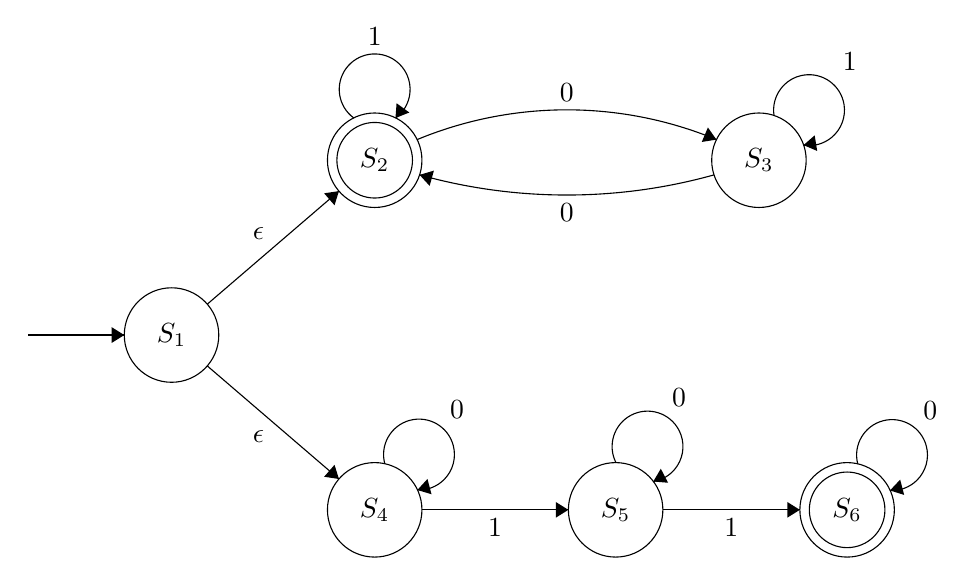
\begin{tikzpicture}[scale=0.2]
	\tikzstyle{every node}+=[inner sep=0pt]
	\draw [black] (17.5,-28.8) circle (3);
	\draw (17.5,-28.8) node {$S_1$};
	\draw [black] (30.4,-17.7) circle (3);
	\draw (30.4,-17.7) node {$S_2$};
	\draw [black] (30.4,-17.7) circle (2.4);
	\draw [black] (54.8,-17.7) circle (3);
	\draw (54.8,-17.7) node {$S_3$};
	\draw [black] (30.4,-39.9) circle (3);
	\draw (30.4,-39.9) node {$S_4$};
	\draw [black] (45.7,-39.9) circle (3);
	\draw (45.7,-39.9) node {$S_5$};
	\draw [black] (60.4,-39.9) circle (3);
	\draw (60.4,-39.9) node {$S_6$};
	\draw [black] (60.4,-39.9) circle (2.4);
	\draw [black] (8.4,-28.8) -- (14.5,-28.8);
	\fill [black] (14.5,-28.8) -- (13.7,-28.3) -- (13.7,-29.3);
	\draw [black] (19.77,-30.76) -- (28.13,-37.94);
	\fill [black] (28.13,-37.94) -- (27.85,-37.04) -- (27.19,-37.8);
	\draw (23.02,-34.84) node [below] {$\epsilon$};
	\draw [black] (19.77,-26.84) -- (28.13,-19.66);
	\fill [black] (28.13,-19.66) -- (27.19,-19.8) -- (27.85,-20.56);
	\draw (23.02,-22.76) node [above] {$\epsilon$};
	\draw [black] (33.096,-16.388) arc (112.48494:67.51506:24.851);
	\fill [black] (52.1,-16.39) -- (51.56,-15.62) -- (51.17,-16.54);
	\draw (42.6,-14) node [above] {$0$};
	\draw [black] (51.949,-18.63) arc (-74.41256:-105.58744:34.791);
	\fill [black] (33.25,-18.63) -- (33.89,-19.33) -- (34.16,-18.36);
	\draw (42.6,-20.41) node [below] {$0$};
	\draw [black] (55.76,-14.87) arc (189:-99:2.25);
	\draw (60.1,-11.45) node [right] {$1$};
	\fill [black] (57.63,-16.74) -- (58.5,-17.11) -- (58.34,-16.12);
	\draw [black] (29.077,-15.02) arc (234:-54:2.25);
	\draw (30.4,-10.45) node [above] {$1$};
	\fill [black] (31.72,-15.02) -- (32.6,-14.67) -- (31.79,-14.08);
	\draw [black] (33.4,-39.9) -- (42.7,-39.9);
	\fill [black] (42.7,-39.9) -- (41.9,-39.4) -- (41.9,-40.4);
	\draw (38.05,-40.4) node [below] {$1$};
	\draw [black] (48.7,-39.9) -- (57.4,-39.9);
	\fill [black] (57.4,-39.9) -- (56.6,-39.4) -- (56.6,-40.4);
	\draw (53.05,-40.4) node [below] {$1$};
	\draw [black] (31.044,-36.982) arc (195.29677:-92.70323:2.25);
	\draw (35.63,-34.14) node [above] {$0$};
	\fill [black] (33.11,-38.64) -- (34.01,-38.91) -- (33.75,-37.94);
	\draw [black] (45.726,-36.912) arc (207.24302:-80.75698:2.25);
	\draw (49.73,-33.37) node [above] {$0$};
	\fill [black] (48.09,-38.1) -- (49.03,-38.18) -- (48.57,-37.29);
	\draw [black] (61.076,-36.989) arc (194.66169:-93.33831:2.25);
	\draw (65.69,-34.19) node [above] {$0$};
	\fill [black] (63.12,-38.67) -- (64.02,-38.95) -- (63.77,-37.98);
	\end{tikzpicture}
\end{center}

\noindent So we have the NFAs for languages $B_1$ and $B_2$.

$\hfill \Box$
\newpage

\section*{Problem 2}
Use the construction given in Theorem 1.39 to convert the following two nondeterministic finite automata to to equivalent deterministic finite automata. \newline

% We use mini pages to put the figures side by side
\begin{minipage}[t]{0.35\linewidth}
	\begin{center}
		(a) \\
		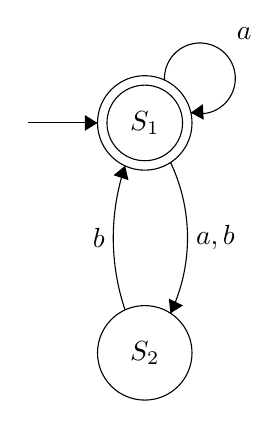
\begin{tikzpicture}[scale=0.2]
		\tikzstyle{every node}+=[inner sep=0pt]
		\draw [black] (23,-14.1) circle (3);
		\draw (23,-14.1) node {$S_1$};
		\draw [black] (23,-14.1) circle (2.4);
		\draw [black] (23,-28.7) circle (3);
		\draw (23,-28.7) node {$S_2$};
		\draw [black] (15.6,-14.1) -- (20,-14.1);
		\fill [black] (20,-14.1) -- (19.2,-13.6) -- (19.2,-14.6);
		\draw [black] (24.634,-16.605) arc (25.41757:-25.41757:11.171);
		\fill [black] (24.63,-26.19) -- (25.43,-25.69) -- (24.53,-25.26);
		\draw (26.22,-21.4) node [right] {$a,b$};
		\draw [black] (21.751,-25.978) arc (-161.35819:-198.64181:14.322);
		\fill [black] (21.75,-16.82) -- (21.02,-17.42) -- (21.97,-17.74);
		\draw (20.5,-21.4) node [left] {$b$};
		\draw [black] (24.254,-11.388) arc (182.91661:-105.08339:2.25);
		\draw (28.81,-8.43) node [right] {$a$};
		\fill [black] (25.92,-13.45) -- (26.74,-13.9) -- (26.69,-12.91);
		\end{tikzpicture}
	\end{center}
\end{minipage}
\begin{minipage}[t]{0.5\linewidth}
	\begin{center}
		(b) \\
		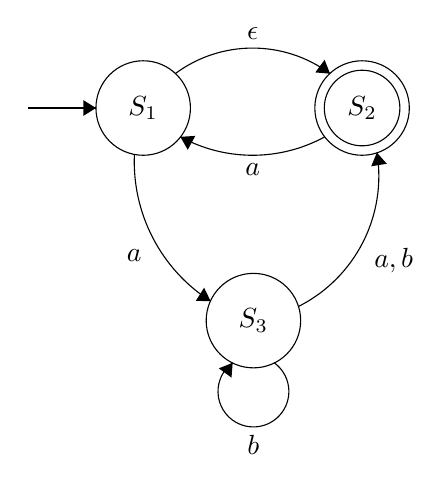
\begin{tikzpicture}[scale=0.2]
		\tikzstyle{every node}+=[inner sep=0pt]
		\draw [black] (17.9,-17.5) circle (3);
		\draw (17.9,-17.5) node {$S_1$};
		\draw [black] (31.8,-17.5) circle (3);
		\draw (31.8,-17.5) node {$S_2$};
		\draw [black] (31.8,-17.5) circle (2.4);
		\draw [black] (24.9,-31) circle (3);
		\draw (24.9,-31) node {$S_3$};
		\draw [black] (10.6,-17.5) -- (14.9,-17.5);
		\fill [black] (14.9,-17.5) -- (14.1,-17) -- (14.1,-18);
		\draw [black] (19.934,-15.318) arc (126.58912:53.41088:8.247);
		\fill [black] (29.77,-15.32) -- (29.42,-14.44) -- (28.83,-15.24);
		\draw (24.85,-13.19) node [above] {$\epsilon$};
		\draw [black] (26.223,-33.68) arc (54:-234:2.25);
		\draw (24.9,-38.25) node [below] {$b$};
		\fill [black] (23.58,-33.68) -- (22.7,-34.03) -- (23.51,-34.62);
		\draw [black] (29.436,-19.327) arc (-61.30057:-118.69943:9.55);
		\fill [black] (20.26,-19.33) -- (20.73,-20.15) -- (21.21,-19.27);
		\draw (24.85,-21) node [below] {$a$};
		\draw [black] (22.178,-29.762) arc (-122.62766:-182.55719:10.515);
		\fill [black] (22.18,-29.76) -- (21.77,-28.91) -- (21.24,-29.75);
		\draw (17.83,-26.89) node [left] {$a$};
		\draw [black] (32.745,-20.334) arc (9.18176:-63.32592:9.28);
		\fill [black] (32.74,-20.33) -- (32.38,-21.2) -- (33.37,-21.04);
		\draw (32.54,-27.16) node [right] {$a,b$};
		\end{tikzpicture}
	\end{center}
\end{minipage}
\newline
\newline
\newline
\noindent
{\bf Proof: } Using the construction theorem, we convert the NFA in (a) to the following DFA:

\begin{center}
	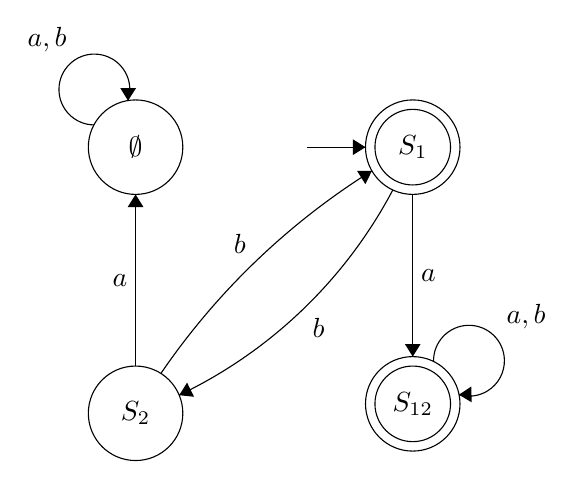
\begin{tikzpicture}[scale=0.2]
	\tikzstyle{every node}+=[inner sep=0pt]
	\draw [black] (14.9,-25) circle (3);
	\draw (14.9,-25) node {$\emptyset$};
	\draw [black] (32.5,-25) circle (3);
	\draw (32.5,-25) node {$S_1$};
	\draw [black] (32.5,-25) circle (2.4);
	\draw [black] (14.9,-41.9) circle (3);
	\draw (14.9,-41.9) node {$S_2$};
	\draw [black] (32.5,-41.3) circle (3);
	\draw (32.5,-41.3) node {$S_{12}$};
	\draw [black] (32.5,-41.3) circle (2.4);
	\draw [black] (12.266,-23.588) arc (269.53768:-18.46232:2.25);
	\draw (9.28,-19.01) node [above] {$a,b$};
	\fill [black] (14.42,-22.05) -- (14.93,-21.25) -- (13.93,-21.25);
	\draw [black] (14.9,-38.9) -- (14.9,-28);
	\fill [black] (14.9,-28) -- (14.4,-28.8) -- (15.4,-28.8);
	\draw (14.4,-33.45) node [left] {$a$};
	\draw [black] (31.234,-27.719) arc (-27.8357:-64.48903:29.909);
	\fill [black] (17.67,-40.75) -- (18.61,-40.85) -- (18.17,-39.95);
	\draw (26.52,-35.81) node [below] {$b$};
	\draw [black] (16.508,-39.368) arc (145.67536:121.99991:45.269);
	\fill [black] (29.91,-26.5) -- (28.96,-26.5) -- (29.49,-27.35);
	\draw (21.52,-31.76) node [above] {$b$};
	\draw [black] (32.5,-28) -- (32.5,-38.3);
	\fill [black] (32.5,-38.3) -- (33,-37.5) -- (32,-37.5);
	\draw (33,-33.15) node [right] {$a$};
	\draw [black] (33.822,-38.62) arc (181.47706:-106.52294:2.25);
	\draw (38.43,-35.79) node [right] {$a,b$};
	\fill [black] (35.43,-40.72) -- (36.24,-41.2) -- (36.22,-40.2);
	\draw [black] (25.8,-25) -- (29.5,-25);
	\fill [black] (29.5,-25) -- (28.7,-24.5) -- (28.7,-25.5);
	\end{tikzpicture}
\end{center}

\newpage
\noindent The NFA in (b) maps to the following DFA under the construction theorem:

\begin{center}
	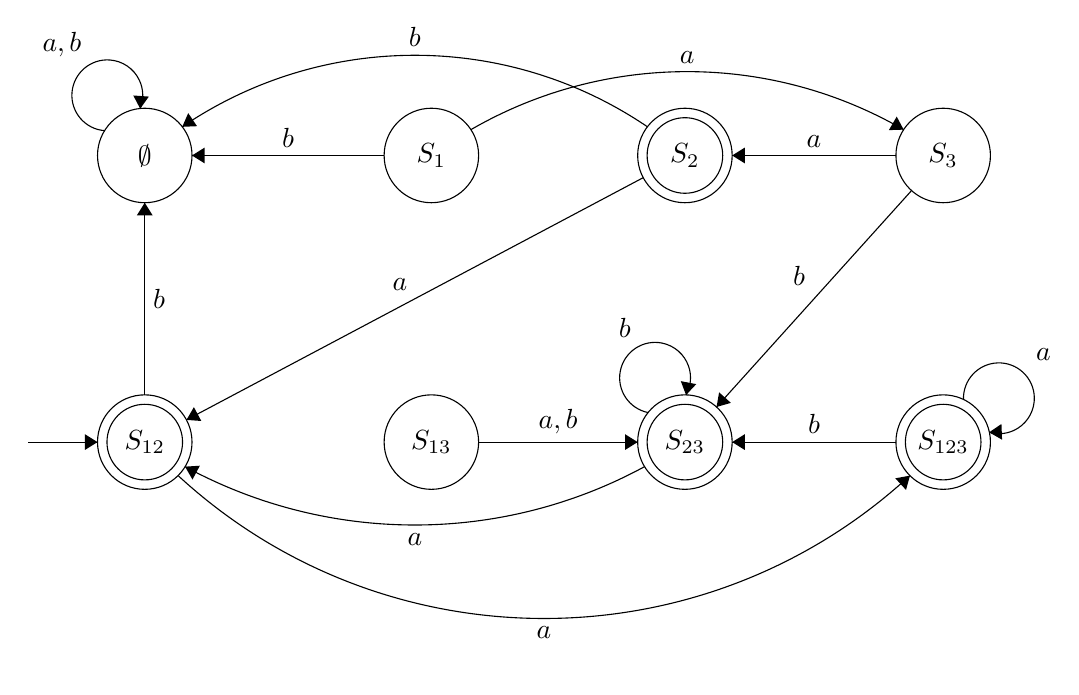
\begin{tikzpicture}[scale=0.2]
	\tikzstyle{every node}+=[inner sep=0pt]
	\draw [black] (11.3,-13.4) circle (3);
	\draw (11.3,-13.4) node {$\emptyset$};
	\draw [black] (29.5,-13.4) circle (3);
	\draw (29.5,-13.4) node {$S_1$};
	\draw [black] (45.6,-13.4) circle (2.4);
	\draw [black] (45.6,-13.4) circle (3);
	\draw (45.6,-13.4) node {$S_2$};
	\draw [black] (62,-13.4) circle (3);
	\draw (62,-13.4) node {$S_3$};
	\draw [black] (11.3,-31.6) circle (2.4);
	\draw [black] (11.3,-31.6) circle (3);
	\draw (11.3,-31.6) node {$S_{12}$};
	\draw [black] (29.5,-31.6) circle (3);
	\draw (29.5,-31.6) node {$S_{13}$};
	\draw [black] (45.6,-31.6) circle (3);
	\draw (45.6,-31.6) node {$S_{23}$};
	\draw [black] (45.6,-31.6) circle (2.4);
	\draw [black] (62,-31.6) circle (3);
	\draw (62,-31.6) node {$S_{123}$};
	\draw [black] (62,-31.6) circle (2.4);
	\draw [black] (8.761,-11.824) arc (265.90016:-22.09984:2.25);
	\draw (6.04,-7.17) node [above] {$a,b$};
	\fill [black] (11.01,-10.43) -- (11.56,-9.66) -- (10.57,-9.59);
	\draw [black] (26.5,-13.4) -- (14.3,-13.4);
	\fill [black] (14.3,-13.4) -- (15.1,-13.9) -- (15.1,-12.9);
	\draw (20.4,-12.9) node [above] {$b$};
	\draw [black] (32.01,-11.76) arc (120.02839:59.97161:27.456);
	\fill [black] (59.49,-11.76) -- (59.05,-10.93) -- (58.55,-11.79);
	\draw (45.75,-7.57) node [above] {$a$};
	\draw [black] (13.68,-11.577) arc (124.17805:55.82195:26.291);
	\fill [black] (13.68,-11.58) -- (14.62,-11.54) -- (14.06,-10.71);
	\draw (28.45,-6.54) node [above] {$b$};
	\draw [black] (42.95,-14.81) -- (13.95,-30.19);
	\fill [black] (13.95,-30.19) -- (14.89,-30.26) -- (14.42,-29.38);
	\draw (27.51,-22) node [above] {$a$};
	\draw [black] (59,-13.4) -- (48.6,-13.4);
	\fill [black] (48.6,-13.4) -- (49.4,-13.9) -- (49.4,-12.9);
	\draw (53.8,-12.9) node [above] {$a$};
	\draw [black] (59.99,-15.63) -- (47.61,-29.37);
	\fill [black] (47.61,-29.37) -- (48.52,-29.11) -- (47.77,-28.44);
	\draw (53.26,-21.04) node [left] {$b$};
	\draw [black] (3.9,-31.6) -- (8.3,-31.6);
	\fill [black] (8.3,-31.6) -- (7.5,-31.1) -- (7.5,-32.1);
	\draw [black] (11.3,-28.6) -- (11.3,-16.4);
	\fill [black] (11.3,-16.4) -- (10.8,-17.2) -- (11.8,-17.2);
	\draw (11.8,-22.5) node [right] {$b$};
	\draw [black] (59.886,-33.727) arc (-47.33094:-132.66906:34.283);
	\fill [black] (59.89,-33.73) -- (58.96,-33.9) -- (59.64,-34.64);
	\draw (36.65,-43.3) node [below] {$a$};
	\draw [black] (32.5,-31.6) -- (42.6,-31.6);
	\fill [black] (42.6,-31.6) -- (41.8,-31.1) -- (41.8,-32.1);
	\draw (37.55,-31.1) node [above] {$a,b$};
	\draw [black] (43.272,-29.726) arc (258.89347:-29.10653:2.25);
	\draw (41.78,-24.97) node [above] {$b$};
	\fill [black] (45.67,-28.61) -- (46.32,-27.92) -- (45.34,-27.73);
	\draw [black] (43.038,-33.159) arc (-61.49073:-118.50927:30.564);
	\fill [black] (13.86,-33.16) -- (14.33,-33.98) -- (14.8,-33.1);
	\draw (28.45,-37.37) node [below] {$a$};
	\draw [black] (59,-31.6) -- (48.6,-31.6);
	\fill [black] (48.6,-31.6) -- (49.4,-32.1) -- (49.4,-31.1);
	\draw (53.8,-31.1) node [above] {$b$};
	\draw [black] (63.29,-28.904) arc (182.15723:-105.84277:2.25);
	\draw (67.87,-26.01) node [right] {$a$};
	\fill [black] (64.92,-30.98) -- (65.74,-31.45) -- (65.7,-30.45);
	\end{tikzpicture}
\end{center}

\noindent However, it should be noted that the above DFA is inefficient since both states $S_1$ and $S_{13}$ have no inputs. The following diagram removes them for simplicity.

\begin{center}
	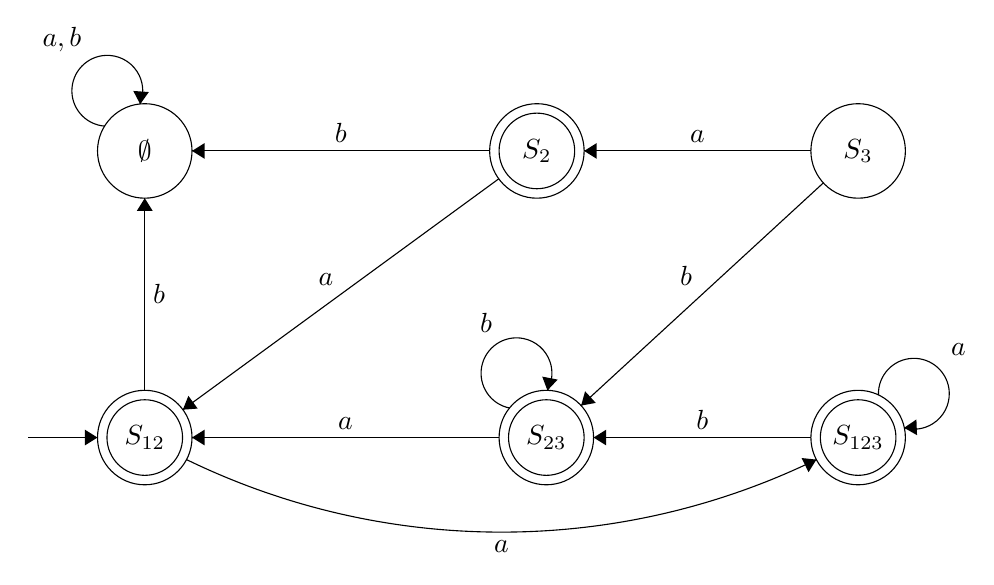
\begin{tikzpicture}[scale=0.2]
	\tikzstyle{every node}+=[inner sep=0pt]
	\draw [black] (11.3,-13.4) circle (3);
	\draw (11.3,-13.4) node {$\emptyset$};
	\draw [black] (36.2,-13.4) circle (2.4);
	\draw [black] (36.2,-13.4) circle (3);
	\draw (36.2,-13.4) node {$S_2$};
	\draw [black] (56.6,-13.4) circle (3);
	\draw (56.6,-13.4) node {$S_3$};
	\draw [black] (11.3,-31.6) circle (2.4);
	\draw [black] (11.3,-31.6) circle (3);
	\draw (11.3,-31.6) node {$S_{12}$};
	\draw [black] (36.8,-31.6) circle (3);
	\draw (36.8,-31.6) node {$S_{23}$};
	\draw [black] (36.8,-31.6) circle (2.4);
	\draw [black] (56.6,-31.6) circle (3);
	\draw (56.6,-31.6) node {$S_{123}$};
	\draw [black] (56.6,-31.6) circle (2.4);
	\draw [black] (8.761,-11.824) arc (265.90016:-22.09984:2.25);
	\draw (6.04,-7.17) node [above] {$a,b$};
	\fill [black] (11.01,-10.43) -- (11.56,-9.66) -- (10.57,-9.59);
	\draw [black] (33.2,-13.4) -- (14.3,-13.4);
	\fill [black] (14.3,-13.4) -- (15.1,-13.9) -- (15.1,-12.9);
	\draw (23.75,-12.9) node [above] {$b$};
	\draw [black] (33.78,-15.17) -- (13.72,-29.83);
	\fill [black] (13.72,-29.83) -- (14.66,-29.76) -- (14.07,-28.95);
	\draw (22.8,-22) node [above] {$a$};
	\draw [black] (53.6,-13.4) -- (39.2,-13.4);
	\fill [black] (39.2,-13.4) -- (40,-13.9) -- (40,-12.9);
	\draw (46.4,-12.9) node [above] {$a$};
	\draw [black] (54.39,-15.43) -- (39.01,-29.57);
	\fill [black] (39.01,-29.57) -- (39.94,-29.4) -- (39.26,-28.66);
	\draw (45.68,-22.01) node [above] {$b$};
	\draw [black] (3.9,-31.6) -- (8.3,-31.6);
	\fill [black] (8.3,-31.6) -- (7.5,-31.1) -- (7.5,-32.1);
	\draw [black] (11.3,-28.6) -- (11.3,-16.4);
	\fill [black] (11.3,-16.4) -- (10.8,-17.2) -- (11.8,-17.2);
	\draw (11.8,-22.5) node [right] {$b$};
	\draw [black] (53.947,-33) arc (-64.05739:-115.94261:45.711);
	\fill [black] (53.95,-33) -- (53.01,-32.9) -- (53.45,-33.8);
	\draw (33.95,-38.11) node [below] {$a$};
	\draw [black] (34.472,-29.726) arc (258.89347:-29.10653:2.25);
	\draw (32.98,-24.97) node [above] {$b$};
	\fill [black] (36.87,-28.61) -- (37.52,-27.92) -- (36.54,-27.73);
	\draw [black] (33.8,-31.6) -- (14.3,-31.6);
	\fill [black] (14.3,-31.6) -- (15.1,-32.1) -- (15.1,-31.1);
	\draw (24.05,-31.1) node [above] {$a$};
	\draw [black] (53.6,-31.6) -- (39.8,-31.6);
	\fill [black] (39.8,-31.6) -- (40.6,-32.1) -- (40.6,-31.1);
	\draw (46.7,-31.1) node [above] {$b$};
	\draw [black] (57.89,-28.904) arc (182.15723:-105.84277:2.25);
	\draw (62.47,-26.01) node [right] {$a$};
	\fill [black] (59.52,-30.98) -- (60.34,-31.45) -- (60.3,-30.45);
	\end{tikzpicture}
\end{center}
	
\noindent So we have the equivalent DFAs for each of the given NFAs.
	
$\hfill \Box$
\newpage

\section*{Problem 3}
Use the procedure described in Lemma 1.55 to convert the following regular expressions to nondeterministic finite automata.
\begin{enumerate}[label=\alph*.]
	\item $(0 \cup 1)^* 000(0 \cup 1)^*$
	\item $(((00)^* (11)) \cup 01)^*$
\end{enumerate}

\noindent
{\bf Proof: } The following NFA diagrams are not at all the simplest ones that could be produced. This is because the it is the result of a proof by construction (which will often produce an inefficient result). We now give the NFA for the regular expression $(0 \cup 1)^* 000(0 \cup 1)^*$:

\begin{center}
	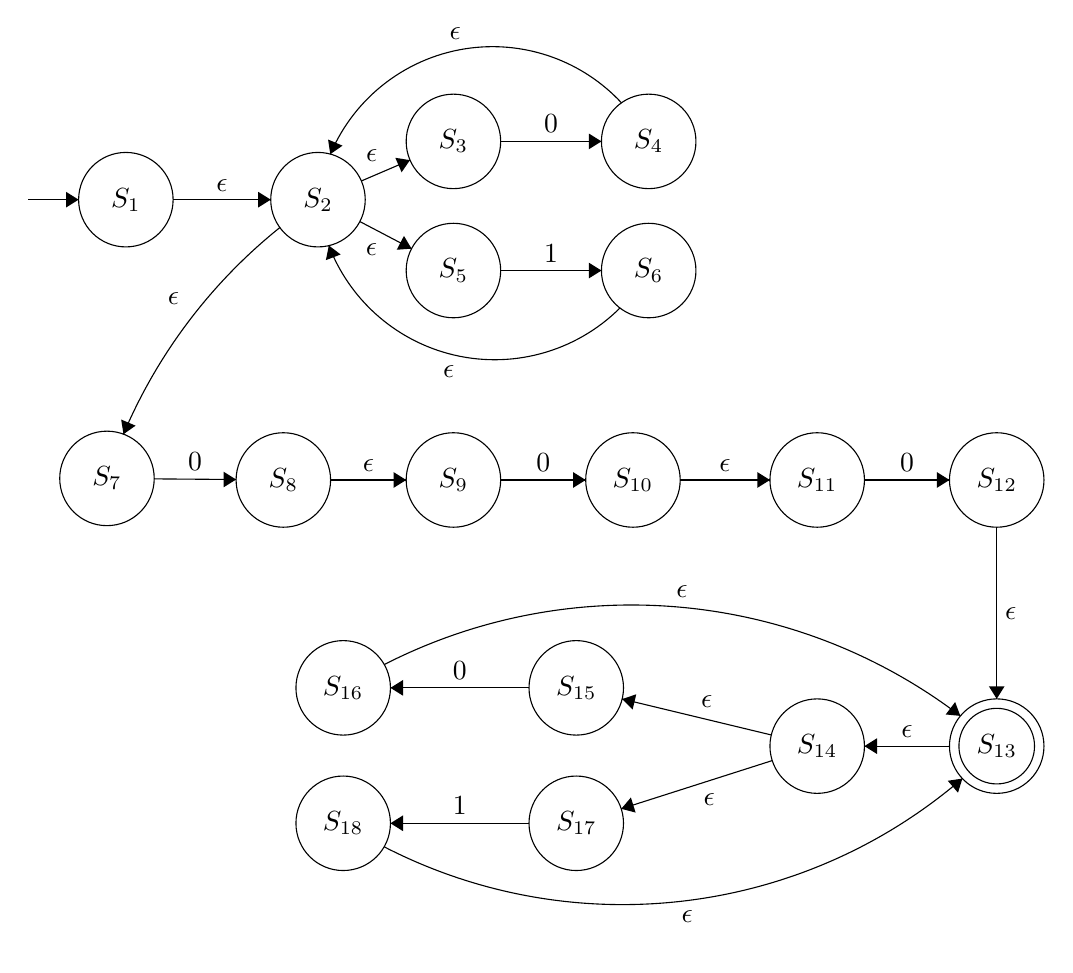
\begin{tikzpicture}[scale=0.2]
	\tikzstyle{every node}+=[inner sep=0pt]
	\draw [black] (10.2,-12.1) circle (3);
	\draw (10.2,-12.1) node {$S_1$};
	\draw [black] (22.4,-12.1) circle (3);
	\draw (22.4,-12.1) node {$S_2$};
	\draw [black] (31,-8.4) circle (3);
	\draw (31,-8.4) node {$S_3$};
	\draw [black] (43.4,-8.4) circle (3);
	\draw (43.4,-8.4) node {$S_4$};
	\draw [black] (31,-16.6) circle (3);
	\draw (31,-16.6) node {$S_5$};
	\draw [black] (43.4,-16.6) circle (3);
	\draw (43.4,-16.6) node {$S_6$};
	\draw [black] (9,-29.8) circle (3);
	\draw (9,-29.8) node {$S_7$};
	\draw [black] (20.2,-29.9) circle (3);
	\draw (20.2,-29.9) node {$S_8$};
	\draw [black] (31,-29.9) circle (3);
	\draw (31,-29.9) node {$S_9$};
	\draw [black] (42.4,-29.9) circle (3);
	\draw (42.4,-29.9) node {$S_{10}$};
	\draw [black] (54.1,-29.9) circle (3);
	\draw (54.1,-29.9) node {$S_{11}$};
	\draw [black] (65.5,-29.9) circle (3);
	\draw (65.5,-29.9) node {$S_{12}$};
	\draw [black] (65.5,-46.8) circle (3);
	\draw (65.5,-46.8) node {$S_{13}$};
	\draw [black] (65.5,-46.8) circle (2.4);
	\draw [black] (54.1,-46.8) circle (3);
	\draw (54.1,-46.8) node {$S_{14}$};
	\draw [black] (38.8,-43.1) circle (3);
	\draw (38.8,-43.1) node {$S_{15}$};
	\draw [black] (24,-43.1) circle (3);
	\draw (24,-43.1) node {$S_{16}$};
	\draw [black] (38.8,-51.7) circle (3);
	\draw (38.8,-51.7) node {$S_{17}$};
	\draw [black] (24,-51.7) circle (3);
	\draw (24,-51.7) node {$S_{18}$};
	\draw [black] (4,-12.1) -- (7.2,-12.1);
	\fill [black] (7.2,-12.1) -- (6.4,-11.6) -- (6.4,-12.6);
	\draw [black] (13.2,-12.1) -- (19.4,-12.1);
	\fill [black] (19.4,-12.1) -- (18.6,-11.6) -- (18.6,-12.6);
	\draw (16.3,-11.6) node [above] {$\epsilon$};
	\draw [black] (25.16,-10.91) -- (28.24,-9.59);
	\fill [black] (28.24,-9.59) -- (27.31,-9.44) -- (27.71,-10.36);
	\draw (25.81,-9.74) node [above] {$\epsilon$};
	\draw [black] (34,-8.4) -- (40.4,-8.4);
	\fill [black] (40.4,-8.4) -- (39.6,-7.9) -- (39.6,-8.9);
	\draw (37.2,-7.9) node [above] {$0$};
	\draw [black] (25.06,-13.49) -- (28.34,-15.21);
	\fill [black] (28.34,-15.21) -- (27.86,-14.4) -- (27.4,-15.28);
	\draw (25.79,-14.85) node [below] {$\epsilon$};
	\draw [black] (34,-16.6) -- (40.4,-16.6);
	\fill [black] (40.4,-16.6) -- (39.6,-16.1) -- (39.6,-17.1);
	\draw (37.2,-16.1) node [above] {$1$};
	\draw [black] (41.581,-18.974) arc (-45.08473:-159.10478:11.275);
	\fill [black] (23.09,-15.01) -- (22.9,-15.94) -- (23.84,-15.58);
	\draw (30.7,-22.59) node [below] {$\epsilon$};
	\draw [black] (23.185,-9.214) arc (157.10513:42.8797:11.18);
	\fill [black] (23.18,-9.21) -- (23.96,-8.67) -- (23.04,-8.28);
	\draw (31.11,-1.97) node [above] {$\epsilon$};
	\draw [black] (10.046,-26.989) arc (157.02363:128.7204:33.653);
	\fill [black] (10.05,-26.99) -- (10.82,-26.45) -- (9.9,-26.06);
	\draw (13.62,-18.41) node [left] {$\epsilon$};
	\draw [black] (12,-29.83) -- (17.2,-29.87);
	\fill [black] (17.2,-29.87) -- (16.4,-29.37) -- (16.4,-30.37);
	\draw (14.6,-29.34) node [above] {$0$};
	\draw [black] (23.2,-29.9) -- (28,-29.9);
	\fill [black] (28,-29.9) -- (27.2,-29.4) -- (27.2,-30.4);
	\draw (25.6,-29.4) node [above] {$\epsilon$};
	\draw [black] (34,-29.9) -- (39.4,-29.9);
	\fill [black] (39.4,-29.9) -- (38.6,-29.4) -- (38.6,-30.4);
	\draw (36.7,-29.4) node [above] {$0$};
	\draw [black] (45.4,-29.9) -- (51.1,-29.9);
	\fill [black] (51.1,-29.9) -- (50.3,-29.4) -- (50.3,-30.4);
	\draw (48.25,-29.4) node [above] {$\epsilon$};
	\draw [black] (57.1,-29.9) -- (62.5,-29.9);
	\fill [black] (62.5,-29.9) -- (61.7,-29.4) -- (61.7,-30.4);
	\draw (59.8,-29.4) node [above] {$0$};
	\draw [black] (65.5,-32.9) -- (65.5,-43.8);
	\fill [black] (65.5,-43.8) -- (66,-43) -- (65,-43);
	\draw (66,-38.35) node [right] {$\epsilon$};
	\draw [black] (62.5,-46.8) -- (57.1,-46.8);
	\fill [black] (57.1,-46.8) -- (57.9,-47.3) -- (57.9,-46.3);
	\draw (59.8,-46.3) node [above] {$\epsilon$};
	\draw [black] (51.18,-46.09) -- (41.72,-43.81);
	\fill [black] (41.72,-43.81) -- (42.38,-44.48) -- (42.61,-43.51);
	\draw (47.09,-44.38) node [above] {$\epsilon$};
	\draw [black] (35.8,-43.1) -- (27,-43.1);
	\fill [black] (27,-43.1) -- (27.8,-43.6) -- (27.8,-42.6);
	\draw (31.4,-42.6) node [above] {$0$};
	\draw [black] (51.24,-47.72) -- (41.66,-50.78);
	\fill [black] (41.66,-50.78) -- (42.57,-51.02) -- (42.27,-50.06);
	\draw (47.25,-49.79) node [below] {$\epsilon$};
	\draw [black] (35.8,-51.7) -- (27,-51.7);
	\fill [black] (27,-51.7) -- (27.8,-52.2) -- (27.8,-51.2);
	\draw (31.4,-51.2) node [above] {$1$};
	\draw [black] (26.608,-41.62) arc (117.08855:52.72179:34.482);
	\fill [black] (63.19,-44.88) -- (62.86,-44) -- (62.26,-44.79);
	\draw (45.51,-37.4) node [above] {$\epsilon$};
	\draw [black] (63.318,-48.858) arc (-49.27792:-117.25434:33.069);
	\fill [black] (63.32,-48.86) -- (62.39,-49) -- (63.04,-49.76);
	\draw (45.85,-57.22) node [below] {$\epsilon$};
	\end{tikzpicture}
\end{center}

\noindent And now we give the NFA for $(((00)^* (11)) \cup 01)^*$:

\begin{center}
	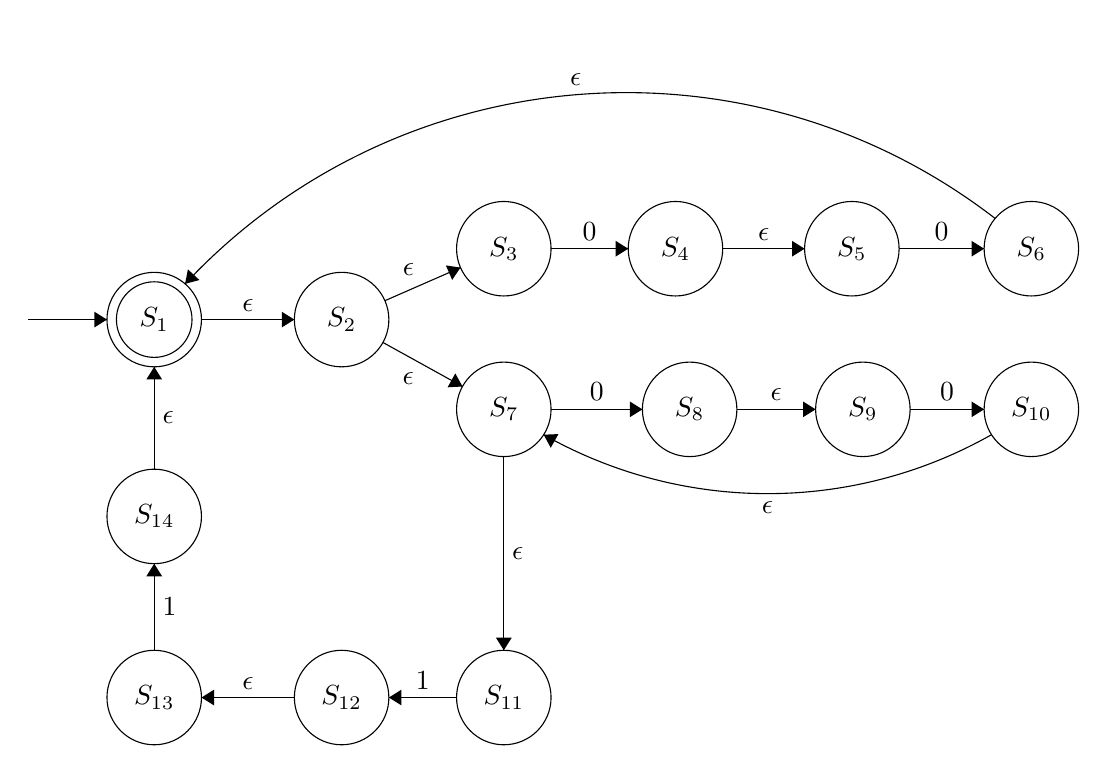
\begin{tikzpicture}[scale=0.2]
	\tikzstyle{every node}+=[inner sep=0pt]
	\draw [black] (15.1,-21.5) circle (3);
	\draw (15.1,-21.5) node {$S_1$};
	\draw [black] (15.1,-21.5) circle (2.4);
	\draw [black] (27,-21.5) circle (3);
	\draw (27,-21.5) node {$S_2$};
	\draw [black] (37.3,-17) circle (3);
	\draw (37.3,-17) node {$S_3$};
	\draw [black] (48.2,-17) circle (3);
	\draw (48.2,-17) node {$S_4$};
	\draw [black] (59.4,-17) circle (3);
	\draw (59.4,-17) node {$S_5$};
	\draw [black] (70.8,-17) circle (3);
	\draw (70.8,-17) node {$S_6$};
	\draw [black] (37.3,-27.2) circle (3);
	\draw (37.3,-27.2) node {$S_7$};
	\draw [black] (49.1,-27.2) circle (3);
	\draw (49.1,-27.2) node {$S_8$};
	\draw [black] (60.1,-27.2) circle (3);
	\draw (60.1,-27.2) node {$S_9$};
	\draw [black] (70.8,-27.2) circle (3);
	\draw (70.8,-27.2) node {$S_{10}$};
	\draw [black] (37.3,-45.5) circle (3);
	\draw (37.3,-45.5) node {$S_{11}$};
	\draw [black] (27,-45.5) circle (3);
	\draw (27,-45.5) node {$S_{12}$};
	\draw [black] (15.1,-45.5) circle (3);
	\draw (15.1,-45.5) node {$S_{13}$};
	\draw [black] (15.1,-34) circle (3);
	\draw (15.1,-34) node {$S_{14}$};
	\draw [black] (7.1,-21.5) -- (12.1,-21.5);
	\fill [black] (12.1,-21.5) -- (11.3,-21) -- (11.3,-22);
	\draw [black] (18.1,-21.5) -- (24,-21.5);
	\fill [black] (24,-21.5) -- (23.2,-21) -- (23.2,-22);
	\draw (21.05,-21) node [above] {$\epsilon$};
	\draw [black] (29.75,-20.3) -- (34.55,-18.2);
	\fill [black] (34.55,-18.2) -- (33.62,-18.06) -- (34.02,-18.98);
	\draw (31.25,-18.74) node [above] {$\epsilon$};
	\draw [black] (29.62,-22.95) -- (34.68,-25.75);
	\fill [black] (34.68,-25.75) -- (34.22,-24.92) -- (33.73,-25.8);
	\draw (31.23,-24.85) node [below] {$\epsilon$};
	\draw [black] (40.3,-17) -- (45.2,-17);
	\fill [black] (45.2,-17) -- (44.4,-16.5) -- (44.4,-17.5);
	\draw (42.75,-16.5) node [above] {$0$};
	\draw [black] (51.2,-17) -- (56.4,-17);
	\fill [black] (56.4,-17) -- (55.6,-16.5) -- (55.6,-17.5);
	\draw (53.8,-16.5) node [above] {$\epsilon$};
	\draw [black] (62.4,-17) -- (67.8,-17);
	\fill [black] (67.8,-17) -- (67,-16.5) -- (67,-17.5);
	\draw (65.1,-16.5) node [above] {$0$};
	\draw [black] (17.062,-19.232) arc (136.89702:52.34076:38.355);
	\fill [black] (17.06,-19.23) -- (17.97,-18.99) -- (17.24,-18.31);
	\draw (41.86,-6.65) node [above] {$\epsilon$};
	\draw [black] (40.3,-27.2) -- (46.1,-27.2);
	\fill [black] (46.1,-27.2) -- (45.3,-26.7) -- (45.3,-27.7);
	\draw (43.2,-26.7) node [above] {$0$};
	\draw [black] (52.1,-27.2) -- (57.1,-27.2);
	\fill [black] (57.1,-27.2) -- (56.3,-26.7) -- (56.3,-27.7);
	\draw (54.6,-26.7) node [above] {$\epsilon$};
	\draw [black] (63.1,-27.2) -- (67.8,-27.2);
	\fill [black] (67.8,-27.2) -- (67,-26.7) -- (67,-27.7);
	\draw (65.45,-26.7) node [above] {$0$};
	\draw [black] (68.27,-28.81) arc (-60.505:-119.495:28.882);
	\fill [black] (39.83,-28.81) -- (40.28,-29.64) -- (40.77,-28.77);
	\draw (54.05,-33.05) node [below] {$\epsilon$};
	\draw [black] (37.3,-30.2) -- (37.3,-42.5);
	\fill [black] (37.3,-42.5) -- (37.8,-41.7) -- (36.8,-41.7);
	\draw (37.8,-36.35) node [right] {$\epsilon$};
	\draw [black] (34.3,-45.5) -- (30,-45.5);
	\fill [black] (30,-45.5) -- (30.8,-46) -- (30.8,-45);
	\draw (32.15,-45) node [above] {$1$};
	\draw [black] (24,-45.5) -- (18.1,-45.5);
	\fill [black] (18.1,-45.5) -- (18.9,-46) -- (18.9,-45);
	\draw (21.05,-45) node [above] {$\epsilon$};
	\draw [black] (15.1,-42.5) -- (15.1,-37);
	\fill [black] (15.1,-37) -- (14.6,-37.8) -- (15.6,-37.8);
	\draw (15.6,-39.75) node [right] {$1$};
	\draw [black] (15.1,-31) -- (15.1,-24.5);
	\fill [black] (15.1,-24.5) -- (14.6,-25.3) -- (15.6,-25.3);
	\draw (15.6,-27.75) node [right] {$\epsilon$};
	\end{tikzpicture}
\end{center}

\noindent So we have the NFAs equivalent to the given regular expressions.

$\hfill \Box$
\newpage

\section*{Problem 4}
Use the procedure described in Lemma 1.60 to convert the following finite automata to regular expressions.

\begin{center}
	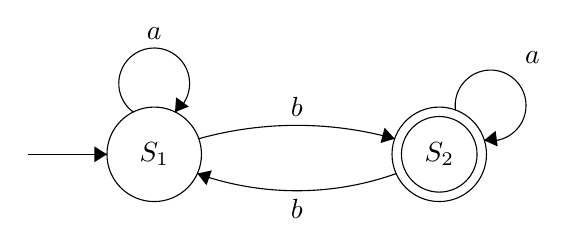
\begin{tikzpicture}[scale=0.2]
	\tikzstyle{every node}+=[inner sep=0pt]
	\draw [black] (30.8,-24) circle (3);
	\draw (30.8,-24) node {$S_1$};
	\draw [black] (48.9,-24) circle (3);
	\draw (48.9,-24) node {$S_2$};
	\draw [black] (48.9,-24) circle (2.4);
	\draw [black] (29.477,-21.32) arc (234:-54:2.25);
	\draw (30.8,-16.75) node [above] {$a$};
	\fill [black] (32.12,-21.32) -- (33,-20.97) -- (32.19,-20.38);
	\draw [black] (22.8,-24) -- (27.8,-24);
	\fill [black] (27.8,-24) -- (27,-23.5) -- (27,-24.5);
	\draw [black] (33.63,-23.01) arc (105.57169:74.42831:23.171);
	\fill [black] (46.07,-23.01) -- (45.43,-22.31) -- (45.17,-23.28);
	\draw (39.85,-21.66) node [above] {$b$};
	\draw [black] (46.165,-25.225) arc (-70.43957:-109.56043:18.861);
	\fill [black] (33.54,-25.22) -- (34.12,-25.96) -- (34.46,-25.02);
	\draw (39.85,-26.81) node [below] {$b$};
	\draw [black] (49.931,-21.195) arc (187.55472:-100.44528:2.25);
	\draw (54.32,-17.88) node [right] {$a$};
	\fill [black] (51.75,-23.11) -- (52.61,-23.5) -- (52.48,-22.51);
	\end{tikzpicture}
\end{center}

\noindent
{\bf Proof: } Using Lemma 1.60, we produce the following GNFA to represent the above DFA.

\begin{center}
	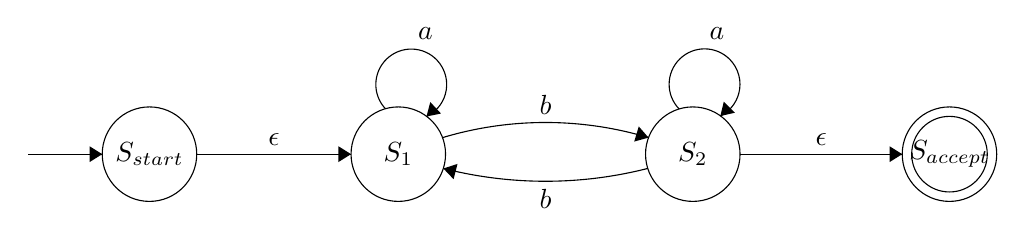
\begin{tikzpicture}[scale=0.2]
	\tikzstyle{every node}+=[inner sep=0pt]
	\draw [black] (13.4,-27) circle (3);
	\draw (13.4,-27) node {$S_{start}$};
	\draw [black] (64.2,-27) circle (3);
	\draw (64.2,-27) node {$S_{accept}$};
	\draw [black] (64.2,-27) circle (2.4);
	\draw [black] (29.2,-27) circle (3);
	\draw (29.2,-27) node {$S_1$};
	\draw [black] (47.9,-27) circle (3);
	\draw (47.9,-27) node {$S_2$};
	\draw [black] (5.7,-27) -- (10.4,-27);
	\fill [black] (10.4,-27) -- (9.6,-26.5) -- (9.6,-27.5);
	\draw [black] (16.4,-27) -- (26.2,-27);
	\fill [black] (26.2,-27) -- (25.4,-26.5) -- (25.4,-27.5);
	\draw (21.3,-26.5) node [above] {$\epsilon$};
	\draw [black] (32.008,-25.95) arc (106.72968:73.27032:22.727);
	\fill [black] (45.09,-25.95) -- (44.47,-25.24) -- (44.18,-26.2);
	\draw (38.55,-24.49) node [above] {$b$};
	\draw [black] (45.042,-27.906) arc (-75.68704:-104.31296:26.259);
	\fill [black] (32.06,-27.91) -- (32.71,-28.59) -- (32.96,-27.62);
	\draw (38.55,-29.22) node [below] {$b$};
	\draw [black] (28.39,-24.124) arc (223.46762:-64.53238:2.25);
	\draw (30.92,-19.78) node [above] {$a$};
	\fill [black] (30.99,-24.61) -- (31.91,-24.42) -- (31.23,-23.69);
	\draw [black] (47.041,-24.138) arc (224.43452:-63.56548:2.25);
	\draw (49.44,-19.76) node [above] {$a$};
	\fill [black] (49.65,-24.58) -- (50.57,-24.37) -- (49.87,-23.66);
	\draw [black] (50.9,-27) -- (61.2,-27);
	\fill [black] (61.2,-27) -- (60.4,-26.5) -- (60.4,-27.5);
	\draw (56.05,-26.5) node [above] {$\epsilon$};
	\end{tikzpicture}
\end{center}

\noindent We then rip $S_2$ to produce

\begin{center}
	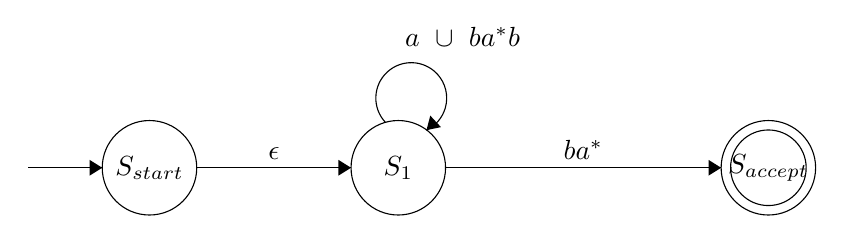
\begin{tikzpicture}[scale=0.2]
	\tikzstyle{every node}+=[inner sep=0pt]
	\draw [black] (13.4,-27) circle (3);
	\draw (13.4,-27) node {$S_{start}$};
	\draw [black] (52.7,-27) circle (3);
	\draw (52.7,-27) node {$S_{accept}$};
	\draw [black] (52.7,-27) circle (2.4);
	\draw [black] (29.2,-27) circle (3);
	\draw (29.2,-27) node {$S_1$};
	\draw [black] (5.7,-27) -- (10.4,-27);
	\fill [black] (10.4,-27) -- (9.6,-26.5) -- (9.6,-27.5);
	\draw [black] (16.4,-27) -- (26.2,-27);
	\fill [black] (26.2,-27) -- (25.4,-26.5) -- (25.4,-27.5);
	\draw (21.3,-26.5) node [above] {$\epsilon$};
	\draw [black] (28.39,-24.124) arc (223.46762:-64.53238:2.25);
	\draw (33.28,-19.36) node [above] {$a\mbox{ }\cup\mbox{ }ba^*b$};
	\fill [black] (30.99,-24.61) -- (31.91,-24.42) -- (31.23,-23.69);
	\draw [black] (32.2,-27) -- (49.7,-27);
	\fill [black] (49.7,-27) -- (48.9,-26.5) -- (48.9,-27.5);
	\draw (40.95,-26.5) node [above] {$ba^*$};
	\end{tikzpicture}
\end{center}

\noindent We then rip $S_1$ which gives

\begin{center}
	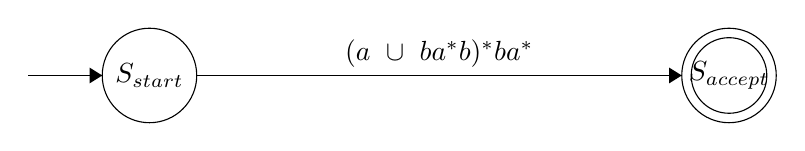
\begin{tikzpicture}[scale=0.2]
	\tikzstyle{every node}+=[inner sep=0pt]
	\draw [black] (15.9,-27) circle (3);
	\draw (15.9,-27) node {$S_{start}$};
	\draw [black] (52.7,-27) circle (3);
	\draw (52.7,-27) node {$S_{accept}$};
	\draw [black] (52.7,-27) circle (2.4);
	\draw [black] (8.2,-27) -- (12.9,-27);
	\fill [black] (12.9,-27) -- (12.1,-26.5) -- (12.1,-27.5);
	\draw [black] (18.9,-27) -- (49.7,-27);
	\fill [black] (49.7,-27) -- (48.9,-26.5) -- (48.9,-27.5);
	\draw (34.3,-26.5) node [above] {$(a\mbox{ }\cup\mbox{ }ba^*b)^*ba^*$};
	\end{tikzpicture}
\end{center}

\noindent So our regular language that corresponds to the given NFA is $(a \cup ba^*b)^* ba^*$.

$\hfill \Box$
\newpage

\section*{Problem 5}
Prove that the following languages are not regular.
\subsection*{5.1} $ A = \{ a^{n^3} \mid n \geq 0 \}$ where $a^x$ means a string of $x$ $a$'s. \\

\noindent
{\bf Proof: } We will prove that $A$ is not regular by contradiction. That is, we will assume that $A$ is regular. Since $A$ is regular, we can apply the pumping lemma. Take $p$ to be the pumping length of $A$. Then, for any string $s \in A$ where $|s| \geq p$ (we know $s$ exists since $p$ is finite and we could construct an element of $A$ to be as large as needed), the following must be true:
\begin{enumerate}
	\item $xy^i z \in A$ $\forall i \geq 0$
	\item $|y| > 0$
	\item $|xy| \leq p$
\end{enumerate}
Choose $s = a^{p^3} \in A$. We then decompose $s = xyz$. By condition 3, it follows that $y$ can consist of no more than the first $p$ letters of $s$. For the case of $i = 2$, we can then write that
$ |s| = |xyz| < |xyyz| = |xyz| + |y|$.
Since $|xyz| = p^3$, we can then say that
$ p^3 < |xyyz| $.
It is also true that
$|xyyz| = |xyz| + |y| = p^3 + |y| \leq p^3 + p$.
We now show some algebra:
$$ p^3 + p < p^3 + 3p^2 + 2p + 1 = (p+1)(p^2 + 2p + 1) = (p + 1)^3$$
We can now truthfully say that $ p^3 < |xyyz| < (p + 1)^3$. Since $p$ is an integer, there is no integer in between $p$ and $p+1$, so $|xyyz|$ cannot be the cube of an integer. Since $|xyyz|$ is not a perfect cube, $xyyz \notin A$. \parspace
We have now shown that $s$ cannot be pumped for $i=2$, which means that the pumping lemma does not apply to $A$. Since the pumping lemma is not true for $A$, the language $A$ cannot be regular.

$\hfill \Box$

\subsection*{5.2} $ B = \{ 0^n 1^m 0^n \mid m,n \geq 0 \}$ \\

\noindent
{\bf Proof: } We will prove that $B$ is not regular by contradiction. That is, we will assume that $B$ is regular. Since $B$ is regular, we can apply the pumping lemma. Take $p$ to be the pumping length of $B$. Then, for any string $s \in B$ where $|s| \geq p$ (we know $s$ exists since $p$ is finite and we construct an element of $B$ to be as large as needed), the following must be true:
\begin{enumerate}
	\item $xy^i z \in B$ $\forall i \geq 0$
	\item $|y| > 0$
	\item $|xy| \leq p$
\end{enumerate}
We now choose $s = 0^p 1 0^p$. Since $B$ is regular, we can decompose $s=xyz$. Because of condition 3, $y$ can consist of no more than the first $p$ letters of $s$ (which are all 0s). Now take $i = 2$. It now must be the case that $xyyz \in B$. Yet, the number of 0s before the 1 (in $s$) is $p + |y|$ while the number of 0s after the 1 (in $s$) is only $p$. By condition 2, $p + |y| > p$ so $xyyz \notin B$. Since $s$ cannot by pumped for $i = 2$, the pumping lemma does not apply to $B$. Since the pumping lemma does not apply to $B$, it must be true that $B$ is non-regular.

$\hfill \Box$

\end{document}